\documentclass[a4paper]{article}

%%%%%%%%%%%%%%%%%%%%%%%%%%%%%%%%%%%%%%%%%%%%%%%%%%%%%%%%%%%%%%%%%%%%%%%%%%%%
% Some common includes. Add additional includes you need.
%%%%%%%%%%%%%%%%%%%%%%%%%%%%%%%%%%%%%%%%%%%%%%%%%%%%%%%%%%%%%%%%%%%%%%%%%%%%
\RequirePackage{ngerman}
\RequirePackage[utf8]{inputenc}
\RequirePackage[T1]{fontenc}
\RequirePackage[margin=30mm,bottom=40mm]{geometry}
\RequirePackage{graphicx}
\RequirePackage{amsmath,amsfonts,amssymb,amsthm}
\RequirePackage{listingsutf8}
\RequirePackage{textcomp}
\RequirePackage{soul}
\RequirePackage{hyperref}
\RequirePackage{tikz}

\renewcommand{\baselinestretch}{1.15} % Line spacing

\usetikzlibrary{arrows.meta}

%%%%%%%%%%%%%%%%%%%%%%%%%%%%%%%%%%%%%%%%%%%%%%%%%%%%%%%%%%%%%%%%%%%%%%%%%%%%
% Defines for mathematical notation. Add additional defines as needed.
%%%%%%%%%%%%%%%%%%%%%%%%%%%%%%%%%%%%%%%%%%%%%%%%%%%%%%%%%%%%%%%%%%%%%%%%%%%%
\def\O{\mathcal{O}}
\def\sort{\mathrm{sort}}
\def\scan{\mathrm{scan}}
\def\dist{\mathrm{dist}}





\newtheorem{theorem}{Satz}


\theoremstyle{definition}
\newtheorem{definition}{Definition}

\theoremstyle{remark}
\newtheorem*{remark}{Bemerkung}

\def\proofname{Beweis}


\usepackage{listings}
\lstset{%
  showstringspaces=false,
  mathescape=true,
  inputencoding=utf8,
  numbers=left,
  xleftmargin=\parindent,
  basicstyle=\footnotesize\ttfamily,
  keywordstyle=\bfseries\color{green!40!black},
  commentstyle=\normalfont\itshape\color{black!60},
  identifierstyle=\color{blue},
  stringstyle=\color{violet},
  tabsize=2%
}


\begin{document}
	\begin{titlepage}
	
	\begin{center}

		\huge \textbf{\textsf{
		\\Arithmetisches Kodieren}} \\
		\LARGE\textbf{\textsc{\\
		Vito Schopper - 7503386
		\\
		Mario Navarro - }}\\ 
		\vspace{2cm}
		\LARGE\textbf{\textsc{\\Pro-Seminar
		\\ Datenkompression WS 2022}}\\ 
		\vspace{2.5cm}
		\large \textbf{
		\\
				Dozent: {Dr.- Ing. The Anh Vuong} \\
Graphische Daten Verarbeitung, Informatik Institut
\\
Goethe Universität , Frankfurt am Main
}
	\end{center}

\end{titlepage}
\tableofcontents\newpage
%\listoffigures\newpage
	
	\section{Thema}
	Hier könnte ein kurzer Satz zur Einleitung stehen.
	
		\section{Theoretische Grundlagen}
	Hier könnte ein kurzer Satz zur Einleitung stehen.
	
		\section{Verfahren-Beschreibung}

	Hier könnte ein kurzer Satz zur Einleitung stehen.
	
		\section{Anwendungsgebiet}
	Hier könnte ein kurzer Satz zur Einleitung stehen.
	
			\section{Qualitätsbewertung über das Verfahren}
	Hier könnte ein kurzer Satz zur Einleitung stehen.
	
			\section{Präsentation / Demonstration Kit}
Wir haben bei der Visualisierung/der Umsetzung des Demonstrations Kit zwischen 2 Fällen unterschieden. Da es bei den Berechnungen während der Kodierung/Dekodierung zu Schwierigkeiten mit den Intervallgrenzen kommt (siehe Verfahren Beschreibung), haben wir ein \textbf{naives} und ein \textbf{genaues} Kit erstellt.
\\
\\
Das naive Kit erstellt eine gut verständliche, visuelle Animation. Jedoch funktioniert dieses Verfahren nur für relativ kleine Eingaben wie z.B ``Hello'' oder ``Laterne''. Bei größeren Eingaben benötigt die Erstellung der Animation erheblich länger. Da dieses Verfahren auch nicht das TODO umsetzt, kommt es hier bei größeren Eingaben zu den in Kapitel 3 erwähnten Rundungsfehlern. Auf kurzen Eingaben ist jedoch eine korrekte
Kodierung/Dekodierung, sowie eine Erstellung einer visuell ansprechenden Animation kein Problem. 
\\
\\
Hierfür haben wir auf das python-Modul \textbf{manim} zurückgegriffen. Dabei handelt es sich um ein Opensource-Projekt des Youtubers ``3Blue1Brown'', welcher es vor mehreren Jahren geschrieben hat, um visuell ansprechende Animationen ifür den Bereich der Mathematik zu erstellen.
\\
Mittlerweile wird dieses Model jedoch durch die Community erweitert und bietet viele Möglichkeiten Themen aus dem MINT-Bereich visuell darzustellen.
\subsection{naives Verfahren}
\subsubsection{Installation}
Es wird das python-modul \textbf{manim}, sowie viele kleine weitere module wie z.B. \textbf{ffmpeg} benötigt, welche jedoch automatisch mit \textbf{manim} heruntergeladen werden.\\
Der Installationsvorgang wird unter \href{https://docs.manim.community/en/stable/installation.html}{https://docs.manim.community/en/stable/installation.html}
genauer beschrieben.
\\
\subsubsection{Kodierung}
Für die Kodierung wird die Datei \textbf{encoding.py} mithilfe des Befehls
\begin{lstlisting}[language=bash,
numbers=none]
manim -pql -v critical encoding.py
\end{lstlisting}
im terminal ausgeführt.
\\
Anschließend wird als Eingabe das zu kodierende Wort erfragt. Hier wie oben erwähnt, kein zu langes Wort eingeben.
Daraufhin kann es je nach länge des Wortes 1-2 min dauern, bis die Animation erstellt
wurde, welche sich direkt in einem neuen Fenster öffnet und angeschaut werden kann.
Alternativ wurde die Animation unter
\begin{lstlisting}[language=bash, numbers=none]
.\SeminarDatenkompression-2022\pythno\media\videos%encodin\480p15\Encoding.mp4
\end{lstlisting}
gespeichert.
\subsubsection{Dekodierung}
Für die Dekodierung wird die Datei \textbf{decoding.py} mithilfe des Befehls
\begin{lstlisting}[language=bash,
numbers=none]
manim -pql -v critical decoding.py
\end{lstlisting}
im terminal ausgeführt.
Anschließend wird als Eingabe zuerst die zu dekodierende Binärzahl
erfragt. Daraufhin wird eine Häufigkeitsverteilung der vorkommenden Buchstaben erfragt.
Diese muss im Format eines python-Dictionaries eingegeben werden.
z.B: TODO: ist Reihenfolge egal?
\begin{lstlisting}[language=bash,
numbers=none]
{"H": 1, "e": 1, "l": 2, "o": 1}
{"A": 1, "e": 1, "f": 2}
\end{lstlisting}
Daraufhin kann es je nach länge des Wortes 1-2 min dauern, bis die Animation erstellt
wurde, welche sich direkt in einem neuen Fenster öffnet und angeschaut werden kann.
Alternativ wurde die Animation unter
\begin{lstlisting}[language=bash,
numbers=none]
.\Seminar-Datenkompression-2022\python%\media\videos\decodin\480p15\Decoding.mp4
\end{lstlisting}
gespeichert.
\\
\\
\subsection{genaues Verfahren}
\subsection{Kodierung}
Für die Kodierung wird eine Eingabe im Eingabefeld erwartet. Falls gewünscht kann man sich mit dem Button \textbf{Generiere Wahrscheinlichkeiten}, die Wahrscheinlichkeitsverteilung der Eingabe anzeigen lassen.


	
	
	
	
% wird am Ende entfernt. Dient nur zur Referenz für gewisse commands

	
	\section{temp}
	wird am Ende entfernt. Dient nur zur Referenz für gewisse commands\\
	Man könnte sich auf Abschnitt \ref{sec:einunterabschnitt} beziehen. Oder auf Formeln
	(\ref{eqn:formel_v}) und (\ref{eqn:formel_e}) und auf Abbildung \ref{fig:bspgraph}.	
	
	\subsection{Ein Unterabschnitt}
	\label{sec:einunterabschnitt}
	Dies ist der Text von einem Unterabschnitt.
	
	\begin{figure}[h]
		\begin{center}
			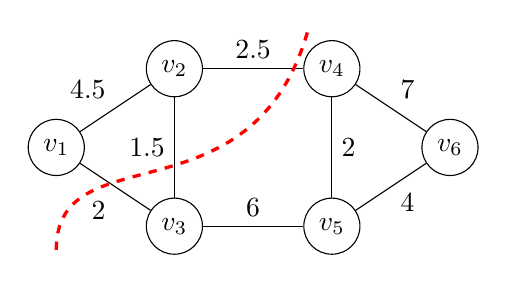
\begin{tikzpicture}
				\node[shape=circle,draw=black] (3) at (0,0) {$v_3$};
				\node[shape=circle,draw=black] (2) at (0,2) {$v_2$};
				\node[shape=circle,draw=black] (4) at (2,2) {$v_4$};
				\node[shape=circle,draw=black] (5) at (2,0) {$v_5$};
				\node[shape=circle,draw=black] (1) at (-1.5,1) {$v_1$};
				\node[shape=circle,draw=black] (6) at (3.5, 1) {$v_6$};
				
				\path [-] (3) edge node[auto] {$1.5$} (2);
				\path [-] (4) edge node[auto] {$2$} (5);
				\path [-] (1) edge node[auto] {$4.5$} (2);
				\path [-] (2) edge node[auto] {$2.5$} (4);
				\path [-] (3) edge node[auto] {$6$} (5);
				\path [-] (1) edge node[auto, left, yshift=-0.3cm] {$2$} (3);
				\path [-] (4) edge node[auto] {$7$} (6);
				\path [-] (5) edge node[auto, right, yshift=-0.2cm] {$4$} (6);
				
				\draw[red, very thick, dashed] (-1.5,-0.3) .. controls (-1.5,1.2) and (1,0) .. (1.7,2.5);
			\end{tikzpicture}
			\caption{Ein Beispielgraph mit eingezeichneter gestrichelter Linie.}
			\label{fig:bspgraph}
		\end{center}
	\end{figure}
	
	\noindent
	Hier könnte auch noch etwas Text stehen.
	
	
	\subsection{Ein weiterer Unterabschnitt}
	Hier könnten Formeln stehen, z.B.
	\begin{align*}
		n^{2} + 2n + 40 = \O(n^{2})
	\end{align*}
	Manchmal möchte man auch Formeln nummerieren, zum Beispiel
	\begin{align}
		V &= \{v_1, \dots, v_n\} \label{eqn:formel_v}\\
		E &= \{\{v_{i}, v_{j}\}\ |\ j \in \{1, \dots, n-1\},\ i = j+1\} \label{eqn:formel_e}
	\end{align}
	

	\begin{remark} ``Pythagoras (geb. um 570 v.Chr.) gilt traditionell als der Entdecker des als Satz des Pythagoras bekannten Lehrsatzes der Euklidischen Geometrie über das rechtwinklige Dreieck. Dieser Satz war schon Jahrhunderte vor Pythagoras den Babyloniern bekannt. Ob sie aber einen Beweis für den Satz kannten, ist unbekannt. Zhmud meint, Pythagoras habe einen Beweis gefunden, während Burkert im Sinne der Schamanismusthese argumentiert, dafür gebe es keinen Beleg und Pythagoras habe sich für mathematische Beweisführung gar nicht interessiert.'' \cite{WIKI}
	\end{remark}
	

	
	\subsection{Der nächste Abschnitt}
	Vielleicht möchte man hierfür eine neue Seite beginnen und Bezug auf \cite{einequelle} oder \cite{eineanderequelle}
	nehmen.
	
		\newpage
	
	\begin{thebibliography}{2}
		\bibitem{einequelle} Namen der Autoren, \textit{Name des Artikels}, Name der Veröffentlichung, Datum, S. 42-46
		\bibitem{eineanderequelle} Namen der anderen Autoren, \textit{Name des anderen Artikels}, Name der anderen Veröffentlichung, Datum, S. 10-20
		\bibitem{WIKI} Wikipedia
	\end{thebibliography}
\end{document}